\documentclass[compress, ucs, xelatex, xcolor=dvipsnames, print,
  hyperref={
    bookmarks=true,
    unicode=true,
    colorlinks=true,
    plainpages=false,
    pdfkeywords={Junak, Pedagogika, Skaut, Skauting, Vychovna metoda},
    linkcolor=Black,
    anchorcolor=Black,
    citecolor=OliveGreen,
    filecolor=OliveGreen,
    menucolor=Black,
    urlcolor=OliveGreen,
    pdftex}
  ]{beamer}

% Nastavení vzhledu
\usecolortheme{spruce}
\useinnertheme[shadow]{rounded}
\useoutertheme{shadow}

\setbeamertemplate{headline} {
  \hbox{%
    \begin{beamercolorbox}[wd=0.5\paperwidth, ht=2.65ex, dp=1.5ex, right]{section in head/foot}
      \insertsectionnavigationhorizontal{0.5\paperwidth}{\hskip0pt plus1fill}{\hskip0pt plus1fill}
      \end{beamercolorbox}%
    \begin{beamercolorbox}[wd=0.5\paperwidth, ht=2.65ex, dp=1.5ex, left]{subsection in head/foot}
      \insertsubsectionnavigationhorizontal{0.5\paperwidth}{}{\hfill\hfill}
      \end{beamercolorbox}%
    }
  \vskip 0pt
  }

\setbeamertemplate{footline} {
  \hbox{%
    \begin{beamercolorbox}[wd=0.333333\paperwidth, ht=2.25ex, dp=1ex, center]{author in head/foot}
      \usebeamerfont{author in head/foot}\insertshortauthor~(\insertshortinstitute)
    \end{beamercolorbox}%
    \begin{beamercolorbox}[wd=0.333333\paperwidth, ht=2.25ex, dp=1ex, center]{title in head/foot}
      \usebeamerfont{title in head/foot}\insertshorttitle
    \end{beamercolorbox}%
    \begin{beamercolorbox}[wd=0.333333\paperwidth, ht=2.25ex, dp=1ex, right]{date in head/foot}
      \usebeamerfont{date in head/foot}\insertshortdate{}\hspace*{2em}
      \insertframenumber{} / \inserttotalframenumber\hspace*{2ex} 
    \end{beamercolorbox}%
    }
  \vskip 0pt
  }

% Další balíčky a nastavení
\usepackage{xltxtra}
\usepackage{metalogo}
\usepackage{xunicode}
\usepackage{fontspec}

\usepackage{multicol}

% Jazyk
\usepackage{polyglossia}
\setdefaultlanguage{czech}

\author{Vojtěch Zeisek}
\institute[Junák --- český skaut]{Ekologický odbor Výkonné rady Junáka --- českého skauta, z.~s.\\
Katedra botaniky Přírodovědecké fakulty UK \&~Botanický ústav AV ČR, v.~v.~i., \href{mailto:zeisek@natur.cuni.cz}{zeisek@natur.cuni.cz}}
\title{Skautská výchovná metoda}
\subtitle{A~její vývoj za poslední století a~desetiletí}
\date{KDF MFF UK 18. 4. 2018}
\titlegraphic{
\includegraphics[width=2.5cm]{lilie.png}}

\begin{document}

\begin{frame}
  \titlepage
\end{frame}

\begin{frame}[allowframebreaks]{Obsah}
  \tableofcontents
\end{frame}

\section{Úvod}

\subsection{Z~historie}

\begin{frame}{Jak to začalo --- velmi stručná historie světového skautingu}
  \begin{itemize}
    \item Skautské hnutí založil britský generál Robert Stephenson Smyth Baden-Powell, pozdější Lord of Gilwell, 1857--1941
    \item Nepřijat na Oxford, 1876 nastupuje na vojenskou akademii a~odjíždí do Indie
    \item Kreslil, hrál divadlo, psal do novin, učil se hindsky, inspiruje se místními stopaři a~zakládá průzkumné oddíly (anglicky \textit{scouts})
    \item 1887 připlouvá do Jižní Afriky, převelen ke zpravodajské službě, později inspektor jezdectva, mj. mapuje Dračí hory, \textbf{sepisuje příručku pro vojenské průzkumníky} (o~pohybu v~přírodě --- později inspirace pro děti pro pobyt v přírodě),~\ldots
    \item 1899--1900 úspěšně brání obležený Mafeking před Búry, povýšen na generálmajora, národní hrdina
    \item Žádá o~propuštění z~armády, \textbf{1907 1. skautský tábor} (Brownsea Island), píše \textbf{Scouting for Boys} (1908)
    \item \textbf{1920 1. světové Jamboree} (setkání) v~Londýně
  \end{itemize}
\end{frame}

\begin{frame}{Robert Baden-Powell}{Co hlavního si pozdější mladý důstojník odnesl ze střední školy\ldots}
  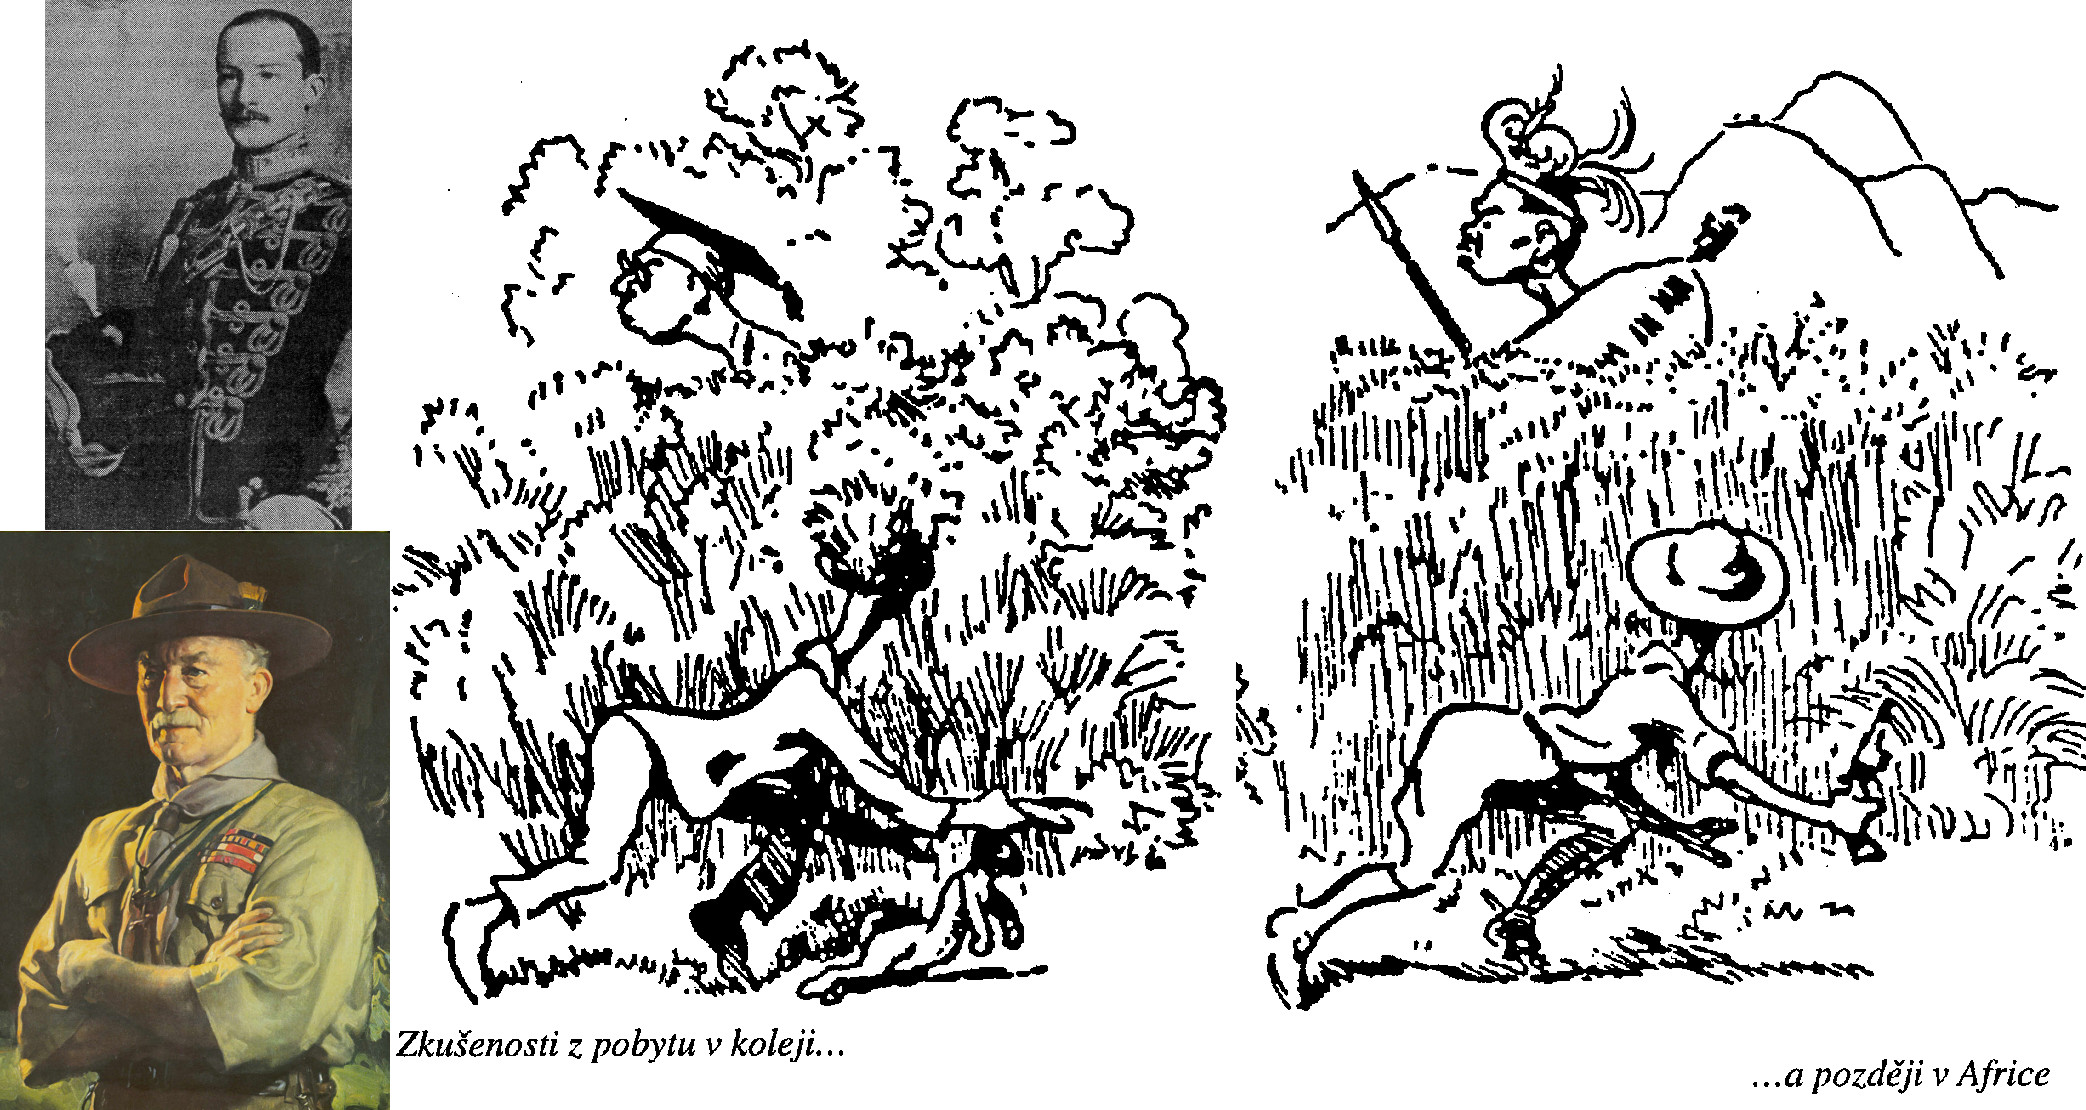
\includegraphics[width=\textwidth]{bp.jpg}
\end{frame}

\begin{frame}{Ernest Thompson Seton (1860--1946)}{Woodcraft a~vliv na český skauting I}
  \begin{multicols}{2}
    \begin{center}
      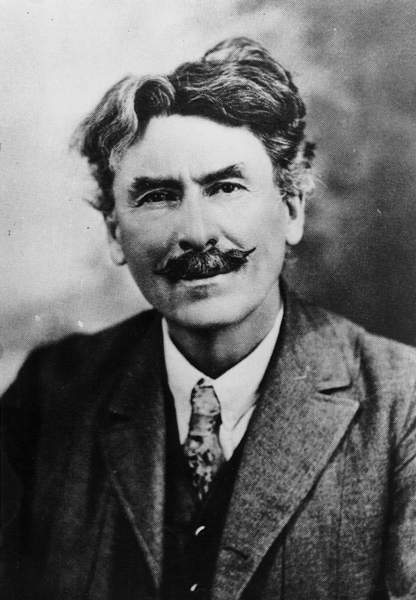
\includegraphics[height=6cm]{seton.jpg}
    \end{center}
    \columnbreak
    \begin{itemize}
      \item Původně anglický malíř, spisovatel, učitel a~přírodovědec
      \item Pracoval v~muzeu, živil se i~psaním článků a knih
      \item Skvělý pozorovatel a~vypravěč o~životě zvířat
      \item Většinu času trávil v~divoké přírodě v~USA, učil se od Indiánů jejich praktickým znalostem a~dovednostem i~filozofii a~pohledu na svět
    \end{itemize}
  \end{multicols}
\end{frame}

\begin{frame}{Ernest Thompson Seton (1860--1946)}{Woodcraft a~vliv na český skauting II}
  \begin{itemize}
    \item 1902 založil \textbf{Woodcraft Indians} --- hnutí inspirující se životem Indiánů (ideou) a snažící se o~výchovu a~poznání
    \begin{itemize}
      \item Znalosti a~respekt k~přírodě
      \item Příroda a~krajina jako zdroj duchovní inspirace
      \item Fyzická zdatnost, rukodělné práce, zručnost
      \item Morální kodex
    \end{itemize}
    \item S~americkou skautskou organizací se rozešel ve zlém, s~Baden-Powellem vycházel velice dobře
    \item Trochu nespravedlivě ve stínu skautingu, jeho hnutí je mnohem menší než to skautské, vzájemně se ovlivňovaly
    \item Mnoho společných prvků se skautingem (práce v~malých skupinách, učení se od ostatních apod.)
    \item Knihy E.~T. Setona měly velký vliv na zakladatele českého skautingu, dále u~nás působí \href{https://www.woodcraft.cz/}{Liga lesní moudrosti} (ta přímo navazuje na jeho americké hnutí)
    \item Skauting klade větší důraz na vztah ke společnosti
  \end{itemize}
\end{frame}

\begin{frame}{Stručná historie českého skautingu I}
  \begin{itemize}
    \item Junáka založil pražský učitel tělocviku \textbf{Antonín Benjamín Svojsík}, 1876--1938
    \item 1909 se dozvěděl o~skautingu, 1911 se vydal do Anglie
    \item \textbf{Ve školním roce 1911/12 založil na žižkovské reálce 1.~skautskou družinu}, reakce veřejnosti byla chladná
    \item 1912 sepisuje \textbf{Základy junáctví}, konzultuje své myšlenky s~intelektuální elitou doby (Drtina, Masaryk, Kramář, Aleš, Jirásek, Rais, Guth-Jarkovský,~\ldots)
    \item 1912 1. skautský tábor u~Lipnice nad Sázavou (šli z~Prahy pěšky), přes celé prázdniny
    \item 1918 skauti pro revoluční Národní výbor zajišťovali kurýrní službu (a~vydávali 1.~známky Republiky Československé)
    \item 1919 založen Svaz junáků --- skautů RČS
    \item Vznikla řada skautských organizací (katoličtí, židovští,~\ldots)
    \item 1939 se skautské organizace spojily do Junáka --- svazu skautů a~skautek RČS
  \end{itemize}
\end{frame}

\begin{frame}{Antonín Benjamín Svojsík a~první čeští skauti}
  \begin{itemize}
    \item Chtěl založit Junáka v~rámci Sokola, nakonec se nedohodli
    \item Na přelomu 19. a~20. století vznikala řada podobných hnutí
  \end{itemize}
  \begin{flushright}
    Kolorované fotografie z~tábora 1912
  \end{flushright}
  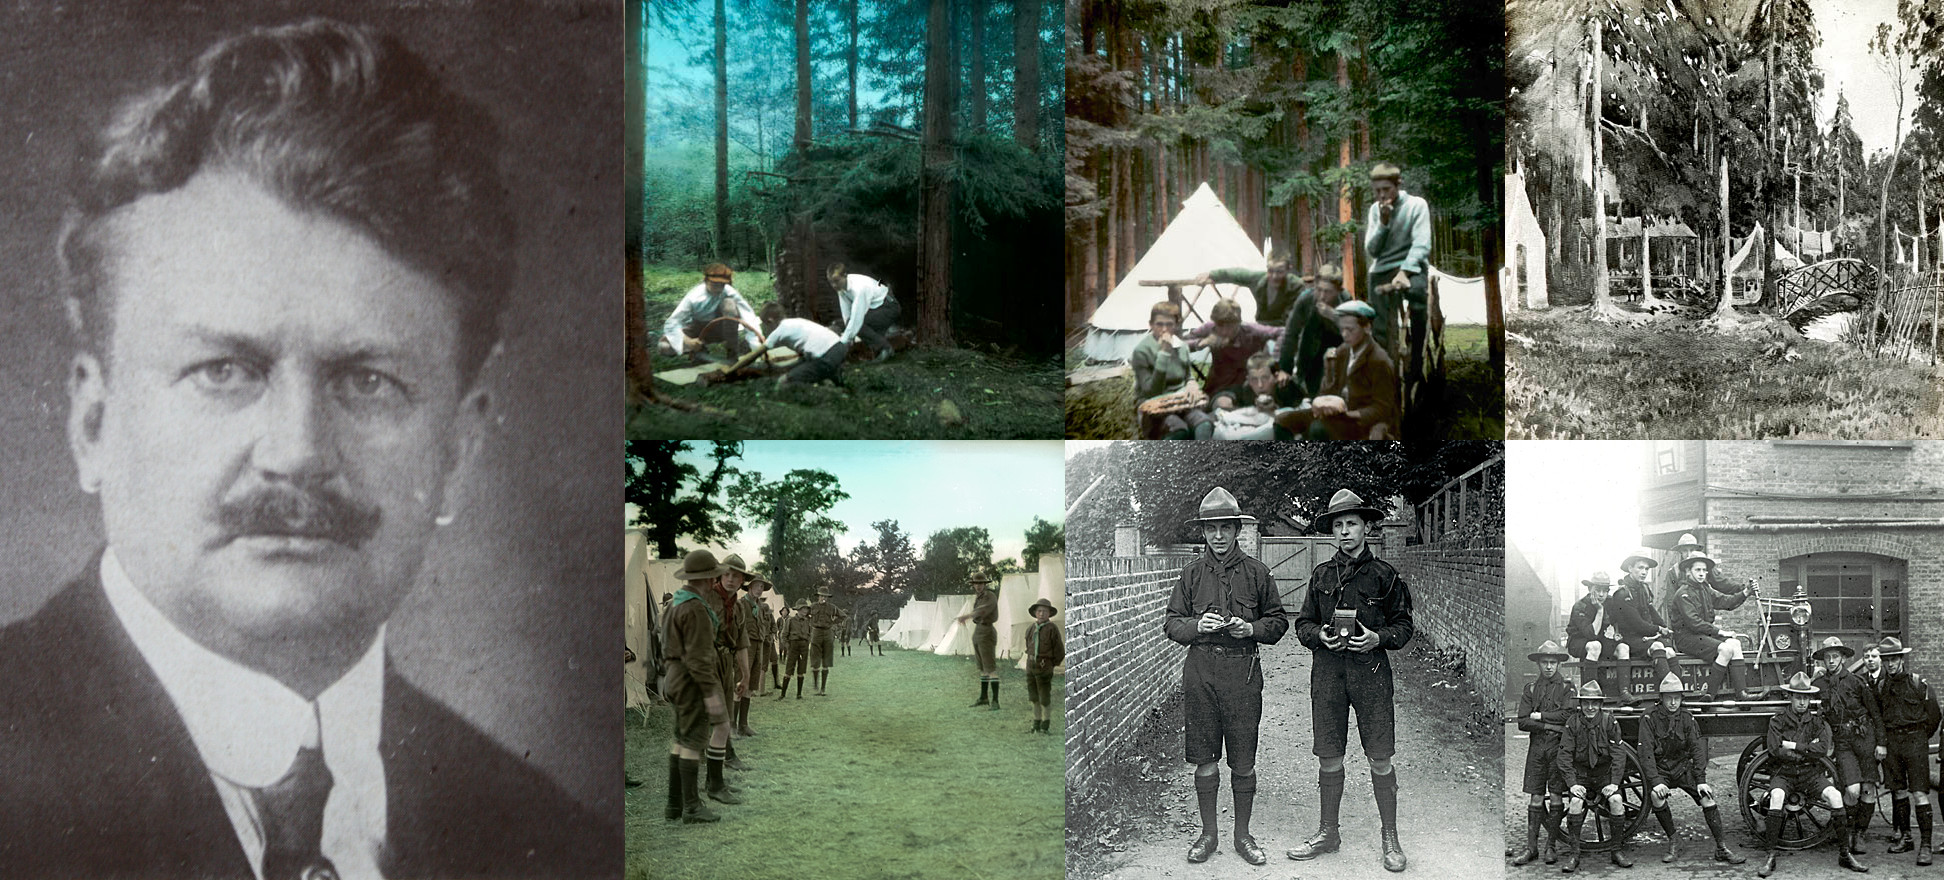
\includegraphics[width=\textwidth]{svojsik_prvni_skauti.jpg}
  \begin{flushright}
    Ostatní snímky pravděpodobně z~20. let
  \end{flushright}
\end{frame}

\begin{frame}{Stručná historie českého skautingu II}
  \begin{itemize}
    \item Za války se skauti zapojili do odboje, zahraničních armád
    \begin{itemize}
      \item Zpravodajská brigáda byla největší (a~velmi úspěšná) odbojová organizace neodhalená Gestapem
    \end{itemize}
    \item 1940 Gestapo rozehnalo řadu táborů, zatýkání představitelů, rozpuštění Junáka (obnoven 1945)
    \item Ihned po únoru 1948 komunisti obsadili ústředí Junáka, vytvořen akční výbor, Junák zlikvidován
    \item 1949 měly vznikat pionýrské oddíly, 1950 Junák formálně zrušen (fakticky již neexistoval)
    \item V~50. letech bylo mnoho skautských činovníků odsouzeno za protikomunistickou činnost, někteří k~smrti
    \item 1968 Junák obnoven
    \item 1969 ÚV KSČ rozhodlo o~vzniku Svazu socialistické mládeže (SSM), 1970 Junák násilně včleněn do SSM
    \item V~70. a~80. letech řada oddílů přežívala pod hlavičkou jiných organizací v~rámci SSM
  \end{itemize}
\end{frame}

\begin{frame}{Junák od 90. let 20. století}
  \begin{itemize}
    \item 1989 obnova Junáka, raketový růst členů
    \item V~90. letech probíhaly debaty o~identitě a~budoucím směřování hnutí a~organizace
    \begin{itemize}
      \item Za totality měl každý svou představu, jak by měl vypadat skauting v~budoucí svobodné společnosti --- trvalo dlouho různé představy sjednotit\ldots
    \end{itemize}
    \item Výsledkem mnohdy bouřlivých debat byl pokles počtu členů a~vznik dalších skautských organizací
    \item Počet členů Junáka nepřetržitě roste od roku 2005 (\href{https://www.skaut.cz/skauting/o-skautingu/fakta-cisla}{nyní přes 60~000~členů})
    \item Díky zákazům během obou totalit nebyl čas na vývoj programu a~reakce na změny společnosti --- do 21. století jsme vstupovali prakticky s~programem z~30. let 20.~století\ldots
    \begin{itemize}
      \item Jak zachovat to dobré a~v~ostatním se zmodernizovat?
    \end{itemize}
    \item Jasně vyplynula potřeba změny dosavadního programu
  \end{itemize}
\end{frame}

\subsection{Myšlenkové základy --- špetka filozofie}

\begin{frame}{Poslání Junáka}{Globální cíl --- čeho chceme dosáhnout}
  \begin{center}
    \begin{Large}
      Posláním Junáka je \textbf{podporovat rozvoj osobnosti} mladých lidí, jejich \textbf{duchovních, mravních, intelektuálních, sociálních a~tělesných schopností} tak, aby byli po celý život připraveni plnit povinnosti k~sobě samým, bližním, vlasti, přírodě a~celému lidskému společenství \textbf{v~souladu s~principy a~metodami}, stanovenými zakladatelem skautského hnutí, lordem Robertem Baden-Powellem a~zakladatelem českého skautingu, prof. Antonínem Benjamínem Svojsíkem.
    \end{Large}
  \end{center}
  \begin{itemize}
    \item Za 1. republiky se na tvorbě skautské metodiky podílely tehdejší špičky psychologie, pedagogiky a~dalších oborů
    \item Hledáme praktické a atraktivní metody, jak toto poslání naplnit --- k tomu slouží výchovný program
  \end{itemize}
\end{frame}

\begin{frame}{Principy skautského hnutí}
  \begin{enumerate}
    \item \textbf{Povinnost k~Bohu}, chápaná jako povinnost hledat v~životě \textbf{vyšší hodnoty než materiální};
    \begin{itemize}
      \item Jde o~morálku, slušnost, dobrotu --- ne nutně o~víru
      \item Skauting je otevřený věřícím různých denominací i ateistům
    \end{itemize}
    \item \textbf{povinnost vůči ostatním}, chápaná jako věrnost své vlasti, která je v~souladu s~úsilím o~mír, o~vzájemné pochopení a~spolupráci mezi lidmi, národy a~různými sociálními skupinami; je pojata jako \textbf{závazek účastnit se na rozvoji společnosti, jako úcta a~láska prokazovaná bližním a~přírodě};
    \begin{itemize}
      \item Nejsme tu jen sami za sebe, ale jsme součástí širšího společenství, na jehož běhu se chceme aktivně podílet, díky své moci máme (jako lidé) zodpovědnost za osud světa
    \end{itemize}
    \item \textbf{povinnost vůči sobě}, chápaná jako odpovědnost za \textbf{rozvoj sebe sama}.
    \begin{itemize}
      \item Nesmíme zapomínat ani na sebe (včetně odpočinku:-)
    \end{itemize}
  \end{enumerate}
\end{frame}

\begin{frame}{Skautský slib a~zákon}
  \begin{multicols}{3}
    \vfill
    \textbf{Slib}
    \vfill
    Slibuji na svou čest, jak dovedu nejlépe: sloužit nejvyšší Pravdě a~Lásce věrně v~každé době, plnit povinnosti vlastní a~zachovávat zákony skautské, duší i~tělem být připraven pomáhat vlasti i~bližním.
    \vfill
    \textit{Dodatek pro věřící:} K~tomu mi dopomáhej Bůh.
    \vfill
    \textbf{Heslo}
    \vfill
    Buď připraven!
    \vfill
    \textbf{Zákon}
    \vfill
    Skaut je
    \begin{enumerate}
      \item pravdomluvný,
      \item věrný a~oddaný,
      \item prospěšný a~pomáhá jiným,
      \item přítelem všech lidí dobré vůle a~bratrem každého skauta,
      \item zdvořilý,
      \item ochráncem přírody a~cenných výtvorů lidských,
      \item poslušný rodičů, představených a~vůdců,
      \item veselé mysli,
      \item hospodárný,
      \item čistý ve slovech, myšlení a~skutcích.
    \end{enumerate}
  \end{multicols}
\end{frame}

\begin{frame}{Cíl skautské výchovy}
  \begin{itemize}
    \item Základní vodítko: principy a~poslání skautského hnutí, skautský slib a~zákon
    \item Výchovné cíle
    \begin{itemize}
      \item Musí být v~souladu se skautskými hodnotami (viz výše)
      \item Musí být praktické --- připravit děti na reálný život
      \begin{itemize}
	\item Neznáme budoucnost --- co bude „praktické“ za 50 let?
      \end{itemize}
      \item Mohou jít proti mainstreamu --- televize,~\ldots
      \item Děti v~oddíle děti průměrně tráví pár hodin týdně na schůzce a~jednou za pár týdnů den/víkend na výpravě --- abychom je mohli pozitivně ovlivnit, musíme tento (oproti škole a~rodině) krátký čas využít maximálně efektivně
    \end{itemize}
    \item Musí to děti bavit
      \begin{itemize}
	\item „Ryby je nutné lovit na to, co chutná rybám a~ne na to, co chutná rybáři.“ (Baden-Powell)
      \end{itemize}
    \item \textbf{Tvrdíme, že máme morální právo ovlivňovat hodnotový žebříček dětí směrem, který považujeme za správný}
  \end{itemize}
\end{frame}

\begin{frame}{Povšimněte si\ldots}
  \begin{itemize}
    \item Zatím jsme neřekli nic o \textit{konkrétní} programové náplni
    \item Skauting je definován „měkkými“ cíly, ne konkrétními činnostmi --- na rozdíl třeba od sportovních klubů, tematických kroužků, apod.
    \item Veřejnost vnímá skauting převážně skrz táboření, ale to je „jen“ výchovný prostředek (viz dále)
    \item Mezi skautskými oddíly je obrovská tematická variabilita --- vodní, suchozemské, inspirujícíc se v historii, věnující se do hloubky nějakému oboru,~\ldots
    \item V činnosti se liší oddíly čistě dívčí, čistě chlapecké, smíšené; vlčácké, skautské a roverské; z vesnic a z velkých měst\ldots
    \item \ldots všem je společný stejný cíl: \textbf{vychovat mladého člověka, který bude platným členem společnosti a bude mít praktické schopnosti a dovednosti pro život v měnícím se světě, za jehož osud cítí (spolu)zodpovědnost a podle toho jedná v souladu s morálními zásadami}
  \end{itemize}
\end{frame}

\section{Metodika}

\subsection{Výchovná metoda}

\begin{frame}{Skautská výchovná metoda\ldots}
  \ldots vede mladého člověka na cestě osobního růstu: soustava výchovy a~sebevýchovy vedoucí k~upevňování charakteru, tvorbě hodnotového systému a~rozvoji dovedností a~znalostí:
  \begin{itemize}
    \item \textbf{Slib a~zákon} --- sebevýchova, dobrovolný závazek
    \item \textbf{Učení se zkušeností} --- praktická i~mravní výchova
    \item \textbf{Družina} --- schopnost být platným členem společenství
    \item \textbf{Symbolický rámec} --- přitažlivé, inspirující a~obohacující
    \item \textbf{Příroda} --- výchovné prostředí, předmět zájmu, ochrany i~citového a~duchovního rozvoje
    \item \textbf{Program osobního růstu} --- pestrý, přitažlivý program i~všestranný individuální rozvoj
    \item \textbf{Dospělí průvodci} --- dospělí ukazují cestu, pomáhají, podporují a~povzbuzují s~respektem k~jedinečnosti dítěte
  \end{itemize}
  Definovaná \href{https://krizovatka.skaut.cz/stredisko/administrativa/novy-obcansky-zakonik-stanovy/nove-stanovy}{ve stanovách}, \href{https://krizovatka.skaut.cz/oddil/program/3360-skautska-vychovna-metoda}{popsaná} a~rozpracovaná v~\href{https://krizovatka.skaut.cz/oddil/program/}{metodických materiálech}.
\end{frame}

\begin{frame}{Historické podoby skautské výchovné metody I}
  \begin{multicols}{2}
    \textit{Základy junáctví}, Svojsík, 1912, 1921, reprint 1991
    \begin{itemize}
      \item Pobyt v~přírodě
      \item Umění pozorovati
      \item Táboření
      \item Noclehování v~přírodě
      \item Škola práce a~rytířství
      \item Fyzický vývoj a~vliv organizace
      \item (Vycházel ze \textit{Scouting for Boys} (Baden-Powell, 1908, česky 2009, \textit{Skauting pro chlapce}), knih Setona a~českých specifik)
    \end{itemize}
    \columnbreak
    \textit{Aids to Scoutmastership}, Baden-Powell, 1920, česky 2006 (\textit{Na pomoc skautským vůdcům})
    \begin{itemize}
      \item Charakterové vlastnosti
      \item Zdraví a~zdatnost
      \item Rukodělné práce a~řemeslné dovednosti
      \item Služba druhým
    \end{itemize}
    \begin{center}
      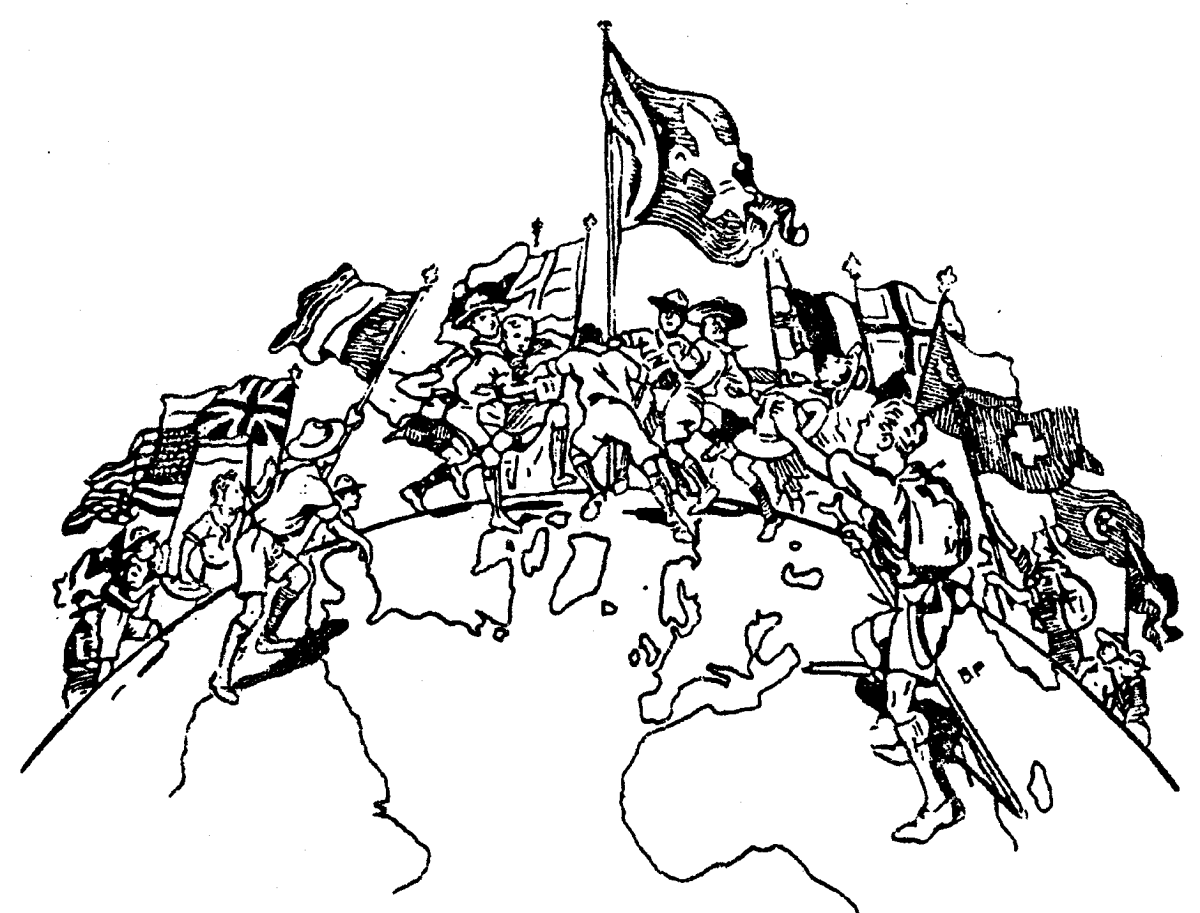
\includegraphics[width=3cm]{sireni.png}
    \end{center}
  \end{multicols}
\end{frame}

\begin{frame}{Historické podoby skautské výchovné metody II}
  \begin{multicols}{2}
    World Organisation of Scout Movement, 1977
    \begin{center}
      
\includegraphics[width=2cm]{wosm.jpg}
    \end{center}
    \begin{itemize}
      \item Slib a~zákon
      \item Učení se zkušeností
      \item Členství v~malých skupinách
      \item Postupný a~stimulující program
    \end{itemize}
  \end{multicols}
  \hrule
  \begin{itemize}
    \item Současná podoba skautské výchovné metody podle WOSM odpovídá té české (respektive naopak), viz \url{https://www.scout.org/method}
    \item Za více jak 100~let se metodika zásadně nezměnila --- posouval se důraz a~detailnost formulace některých bodů
    \item \href{https://www.scout.org/}{WOSM} sdružuje skauty i~skautky, \href{https://www.wagggs.org/}{WAGGGS} jen skautky, \href{http://www.isgf.org/}{ISGF} dospělé --- jejich metodiky se zásadně neliší
  \end{itemize}
\end{frame}

\subsection{Čas na změnu}

\begin{frame}{Proč nový program po roce 2000?}
  \begin{itemize}
    \item Změna společnosti
    \begin{itemize}
      \item Konzum, zrychlená doba, vliv médií, internetu, techniky,~\ldots
      \item Děti rychleji dospívají a~baví je jiné věci, než v~minulosti
    \end{itemize}
    \item Historický vývoj Junáka (zákazy,~\ldots) --- od 1. republiky do přelomu tisíciletí se moc nezměnil\ldots
    \item V~hnutí byla patrná nespokojenost se stavem programu
    \item Charta českého skautingu (2005) --- obecné cíle rozvoje
    \begin{itemize}
      \item Odkazuje na historické kořeny, uvědomuje si současný svět a~otevírá skauting pro budoucnost
    \end{itemize}
    \item Inspirace u skautských organizací, které si podobným procesem prošly dříve (Irsko, Slovensko,~\ldots)
  \end{itemize}
  \begin{center}
    \begin{tabular}{ll}
      \textbf{„Starý program“} & \textbf{„Nový program“}\\
      Jednotlivé dílčí úkoly. & Komplexní úkoly, projekty.\\
      Hlavně o~znalostech. & Něco dokázat, udělat.\\
      Stejná úroveň pro všechny. & Nastavitelná obtížnost.\\
      Bez kontextu a~návaznosti. & Provázaný, motivační, atraktivní.
    \end{tabular}
  \end{center}
\end{frame}

\subsection{Program}

\begin{frame}{Výchovné kategorie}{Každá má svá specifika, základní principy se příliš nemění\ldots}
  \begin{itemize}
    \item \href{https://krizovatka.skaut.cz/oddil/program/benjaminci}{Benjamínci} --- předškolní děti
    \item \href{https://krizovatka.skaut.cz/oddil/program/svetlusky-a-vlcata}{Světlušky a vlčata} --- mladší školní věk (cca 1. stupeň ZŠ)
    \item \href{https://krizovatka.skaut.cz/oddil/program/skautky-a-skauti}{Skautky a skauti} --- starší školní věk (cca 2. stupeň ZŠ)
    \item \href{https://krizovatka.skaut.cz/oddil/program/rangers-a-roveri}{Rangers a roveři} --- cca střední škola, počátek vysoké
    \item \href{https://krizovatka.skaut.cz/oddil/program/rodinny-skauting}{Rodinný skauting} --- tábory (bývalých) vedoucích s malými dětmi
    \item \href{https://krizovatka.skaut.cz/oddil/program/dospeli}{Oldskauti} --- dospělí
  \end{itemize}
\end{frame}

\begin{frame}{Výchovný program}
  \begin{itemize}
    \item Výsledek skautské výchovy --- výchovné cíle skautingu
    \begin{itemize}
      \item Mladý člověk cca na konci střední až počátku vysoké školy
      \item Dovednosti, schopnosti a~postoje, které má mladý člověk ovládat --- koho chceme vychovat
    \end{itemize}
    \item Skautská metoda
    \item Věkové kategorie
    \item Výchovné nástroje
    \item Metodické příručky pro vedoucí
    \item Hodnocení kvality oddílu a~výchovného dopadu
    \item Management, lidské zdroje, found rising,~\ldots
    \item Velká reforma výchovného programu: 2005--2013
    \begin{itemize}
      \item Vlastně nikdy nekončí\ldots
      \item Od podzimu 2016 jeho vyhodnocení a~začátek prací na úpravách\ldots
    \end{itemize}
  \end{itemize}
\end{frame}

\begin{frame}{Jak při tvorbě výchovného programu postupujeme}
  \begin{enumerate}
    \item Definování obecných cílů (kompetence)
    \item Rozpracování dílčích cílů (podle věku,~\ldots)
    \item Výběr vhodných indikátorů (jak poznáme, je-li cíl splněn)
    \item Tvorba programů vedoucích ke splnění cílů
  \end{enumerate}
  \begin{itemize}
    \item Obecné cíle se definovaly na začátku pro všechny věkové kategorie
    \item Rozpracování obecných cílů se provádí pro jednotlivé věkové kategorie (dílčí cíle)
    \item Další nástroje sloužící k~motivaci,~\ldots
    \item Postupná tvorba databáze programů
    \item Metodická podpora pro vedoucí a~další „uživatelská“ podpora vedoucím oddílů ze strany organizace
  \end{itemize}
\end{frame}

\begin{frame}{Co chceme, aby uměl mladý člověk poté, co projde naší výchovou a~na prahu dospělosti odejde?}
  \begin{center}
    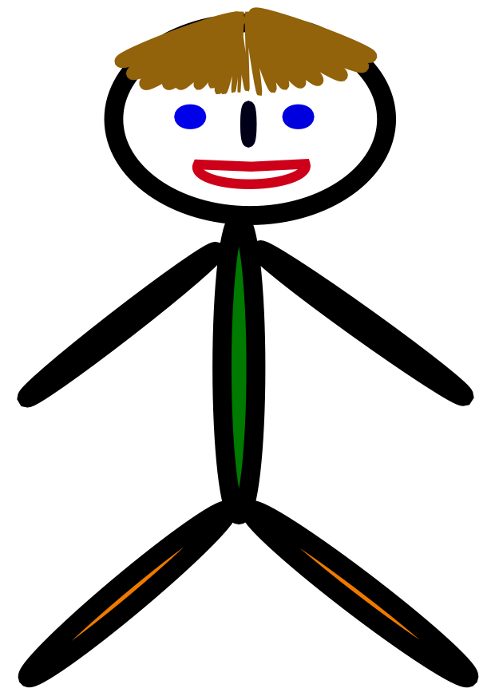
\includegraphics[height=6.5cm]{pepicek.png}
  \end{center}
\end{frame}

\subsection{Kompetence}

\begin{frame}{Skauting a~klíčové kompetence}
  \begin{center}
    Klíčové kompetence: přenosný a~univerzálně použitelný \textbf{soubor vědomostí, dovedností a~postojů}, které potřebuje každý jedinec \textbf{pro své osobní naplnění a~rozvoj, pro zapojení se do společnosti} a~úspěšnou zaměstnatelnost.
  \end{center}
  \begin{itemize}
    \item Kompetence je souborem schopností, dovedností, znalostí a~postojů vztahující se k~určité oblasti
    \item Kompetence se rovnají výchovným záměrům
    \item Jsou rozpracované pro jednotlivé kategorie
    \item Navazují na ně výchovné cíle a~metody
    \item Úspěšnost definují indikátory (ukazatele, zda dochází k~rozvoji dané kompetence)
    \item Jsou zpracovávány a~konzultovány s~odborníky na danou oblast (i~mimo Junáka)
  \end{itemize}
\end{frame}

\begin{frame}{Seznam kompetencí}
  \begin{enumerate}
    \item Duchovní kompetence
    \begin{itemize}
      \item Láska, svědomí, meditace, globální zodpovědnost
      \item V~podstatě jde o~morálku v~nejširším smyslu
    \end{itemize}
      \item Psychologické (vztahové)
    \begin{itemize}
      \item Já (k~sobě), já a~ty, já a~my, já a~společnost
      \item Sociální dovednosti, začlenění se do společnosti
    \end{itemize}
    \item Manažerské
    \begin{itemize}
      \item Sám sobě manažerem, práce s~informacemi a~řešení problému, vlastní názor, odolávání manipulaci, prezentace na veřejnosti, týmová práce, komunikace
    \end{itemize}
    \item Občanské (enviromentální)
    \begin{itemize}
      \item Krása -- vnímání a~vytváření, krása a~jedinečnost přírody, vztah k~přírodě, vztah ke krajině, vědomí provázanosti, respekt k~různosti, aktivní občan
      \item Ochrana přírody díky lásce k~ní, aktivní přístup ke světu
    \end{itemize}
    \item Praktické dovednosti
    \begin{itemize}
      \item Přežití v~přírodě, osobní dovednosti, společenské dovednosti, řešení krizových situací
    \end{itemize}
  \end{enumerate}
\end{frame}

\begin{frame}{Příklad rozpracování jedné kompetence}
  \begin{itemize}
    \item Kompetence
    \begin{itemize}
      \item Má dovednosti a~nástroje pro praktický život, umí použít „pracovní nástroje“ své doby (politické, finanční, mediální\ldots)
    \end{itemize}
    \item Výchovný cíl
    \begin{itemize}
      \item Dokáže hospodařit s~penězi (8--10 let)
    \end{itemize}
    \item Metody
    \begin{itemize}
      \item Hry, ve kterých jsou použity peníze pro nákup potřebných surovin („budovatelské strategie“,~\ldots)
      \item Nakupování potravin a~jiných věcí pro oddíl
      \item Vedení pokladny družiny, vybírání peněz na výpravě
    \end{itemize}
    \item Indikátory
    \begin{itemize}
      \item Šetří si nějaké peníze se svého kapesného
      \item Nekupuje si zbytečnosti
      \item Bezchybně vrátí peníze po nákupu
    \end{itemize}
  \end{itemize}
\end{frame}

\section{Stezka}

\subsection{Struktura}

\begin{frame}{Oblasti stezky}
  \begin{itemize}
    \item Moje dovednosti a~znalosti
    \begin{itemize}
      \item Praktický život, fyzická zdatnost, buď připraven, hledání řešení, vyjadřování, zručnost
    \end{itemize}
    \item Kdo jsem?
    \begin{itemize}
      \item Já a~můj život, moje svědomí, osobní rozvoj
    \end{itemize}
    \item Můj kamarád
    \begin{itemize}
      \item Vztahy mezi lidmi, moje vztahy, komunikace mezi lidmi, pomoc druhým
    \end{itemize}
    \item Můj domov
    \begin{itemize}
      \item Moje rodina, moje parta, družina jako tým
    \end{itemize}
    \item Svět okolo nás
    \begin{itemize}
      \item Já a~demokracie, já občan, propojený svět, různost světa, příběhy našeho světa
    \end{itemize}
    \item Příroda kolem nás
    \begin{itemize}
      \item Pobyt v~přírodě, vnímání přírody, poznávání přírody, hodnota přírody, šetrné chování
    \end{itemize}
  \end{itemize}
  \alert{Smysl užívání kompetencí: \textbf{proměnit skautské principy v~život}}
\end{frame}

\begin{frame}{Stezka pro skautský věk}
  \begin{itemize}
    \item Jeden ze základních výchovných nástrojů --- je všestranná, rozličná a~vyžaduje osobní zapojení vedoucích i~dětí
    \item V~současnosti probíhá revize na základě zpětné vazby z~hnutí
  \end{itemize}
  \begin{center}
    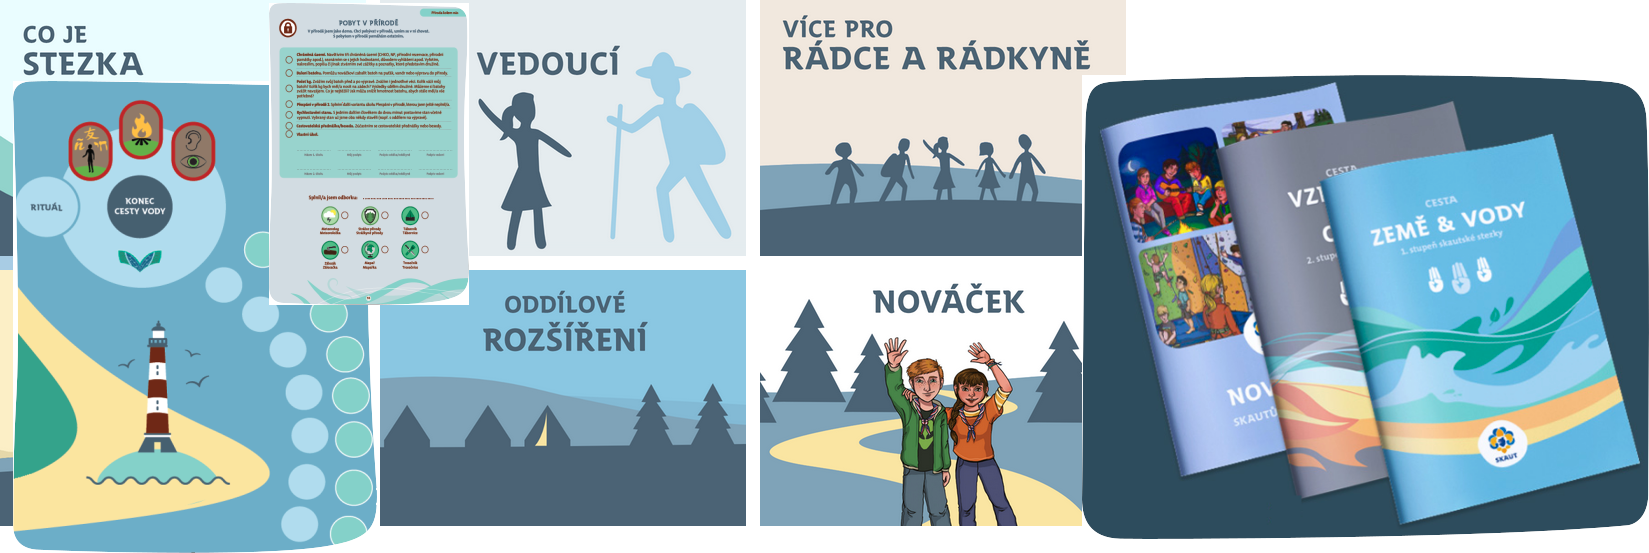
\includegraphics[height=5.5cm]{stezka.png}
  \end{center}
\end{frame}

\begin{frame}{Stezka nejsou jen 4~sešity}
  \begin{multicols}{2}
    \begin{itemize}
      \item Propracovaný systém nástrojů a~motivačních prvků
      \item Prostředek k~dosahování výchovných cílů
      \item Hlavní průvodce na cestě osobního rozvoje
      \item Vede k~osobnímu rozvoji
      \item Obsahuje program zajímavý pro dnešní děti
      \item Má atraktivní a~srozumitelnou formu
      \item Čtyři stupně (věkové kategorie) --- čtyři živly
      \item Ke stažení \href{https://krizovatka.skaut.cz/oddil/program/skautky-a-skauti/skauti-skautky-stezky}{skautské} i~\href{https://krizovatka.skaut.cz/oddil/program/svetlusky-a-vlcata}{vlčácké}
    \end{itemize}
    \columnbreak
    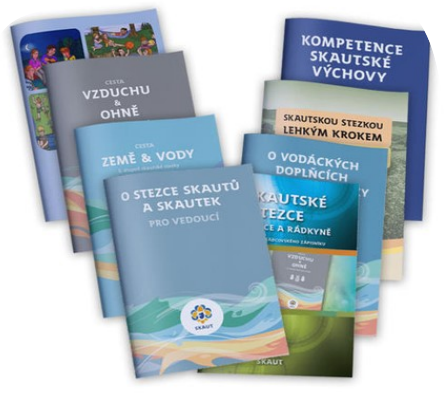
\includegraphics[height=7cm]{stezky.png}
  \end{multicols}
\end{frame}

\subsection{Související nástroje}

\begin{frame}{Nováček --- pro začátek}
  \begin{multicols}{2}
    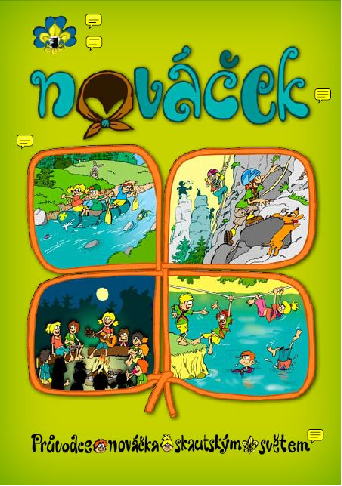
\includegraphics[height=7cm]{novacek.png}
    \columnbreak
    \begin{itemize}
      \item Uvede nováčka do oddílu
      \item Zábavná forma
      \item Seznámí se skautingem a~vším, co k~němu patří
      \item Oddílové doplňky --- variabilní
      \item Varianty pro světlušky, vlčata, vodní i~suchozemské skauty a~skautky
      \item \href{https://krizovatka.skaut.cz/oddil/program/skautky-a-skauti/skauti-skautky-stezky/novacek}{Ke stažení v~různých variantách}
      \item Oddíly si jej mohou upravit podle svých potřeb
    \end{itemize}
  \end{multicols}
\end{frame}

\begin{frame}{Skautské výzvy --- něco velkého, nevšedního}
  \begin{multicols}{2}
    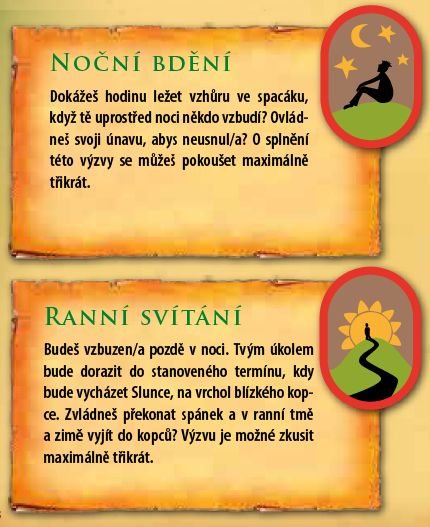
\includegraphics[height=6.1cm]{vyzvy.png}
    \begin{itemize}
      \item Po splnění stupně privilegovaná možnost plnit si jednu výzvu
      \begin{itemize}
	\item Noční bdění
	\item Ranní svítání
	\item Výsadek
	\item Noční návrat
	\item Tři orlí pera
	\item Dva dny bez ničeho
	\item 24 hodin na stromech
      \end{itemize}
      \item \href{https://krizovatka.skaut.cz/oddil/program/skautky-a-skauti/skauti-skautky-stezky/skauti-skautky-stezky-vyzvy}{Kompletní seznam je on-line}
    \end{itemize}
  \end{multicols}
\end{frame}

\begin{frame}{Odborky}
  \begin{itemize}
    \item Stezky pokrývají +/- společný základ, kterým by si (s určitou individualizací) měli projít všichni
    \item Odborky reflektují šíři tématického záběru různých oddílů --- umožňují dětem rozvíjet se v nějaké oblasti (jsou vodítkem na cestě k určité odbornosti)
    \item Není účelem nahradit specializované kroužky, ale dát dětem prostor pro rozvoj individuálních zájmů
    \item Velký důraz je kladen na sdílení znalostí s oddílem --- vzájemné učení se
    \item Pro přehled viz \url{https://odborky.skaut.cz/}
  \end{itemize}
  \begin{center}
    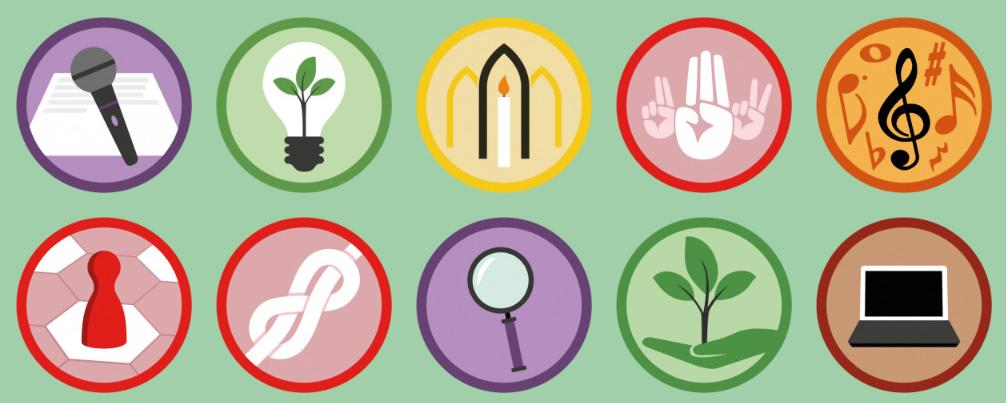
\includegraphics[height=2cm]{odborky.jpg}
  \end{center}
\end{frame}

\subsection{Práce se stezkou}

\begin{frame}{Výhody stezky}
  \begin{itemize}
    \item Všestrannost, rozličnost a~osobní zapojení
    \item Stezka je vodítkem pro vytváření celoročního programu
    \item Stezka umožňuje snadné přizpůsobení oddílu
    \item Propracovaný nástroj osobního rozvoje
    \item Zatraktivnění programu
    \item Během historie skautingu měla a~má mnoho podob
  \end{itemize}
  \begin{center}
    
\includegraphics[height=4cm]{im-possible_m.png}
  \end{center}
\end{frame}

\begin{frame}{Pravidla a~plnění stezky}
  \begin{itemize}
    \item Výběr aktivit
    \begin{itemize}
      \item Některé jsou povinné
      \item Vybírá se po konzultaci s~vedoucím (neplní se všechny)
      \item Lze je plnit v~libovolném pořadí
      \item Aktivitu lze upravit, vymyslet,~\ldots
    \end{itemize}
    \item Kdo hodnotí
    \begin{itemize}
      \item Dítě a~dvě další osoby (vedoucí, rádce, rodič, externí odborník,~\ldots)
    \end{itemize}
    \item Hodnocení
    \begin{itemize}
      \item Musí se shodnout dítě a~další hodnotitel(é)
    \end{itemize}
    \item Plnění
    \begin{itemize}
      \item Přímé plnění
      \item Nepřímé plnění
      \item Přímé plnění s~přípravou
      \item Pro některé body nejsou vhodné všechny způsoby
    \end{itemize}
  \end{itemize}
\end{frame}

\begin{frame}{Stezka zdaleka není vše\ldots}{Některé nástroje fungují lépe, jiné hůře a~čekají je změny\ldots}
  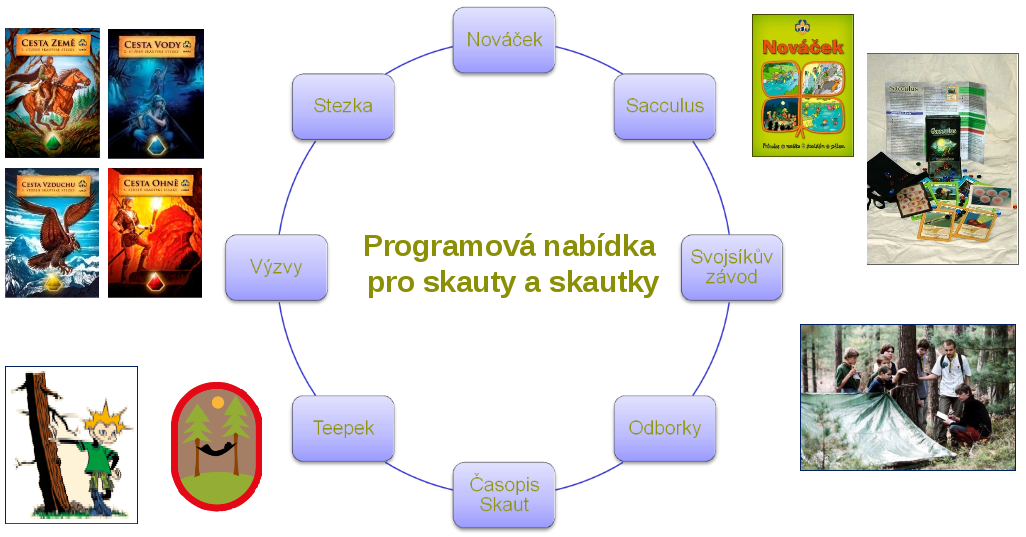
\includegraphics[width=\textwidth]{komplet.png}
\end{frame}

\section{Revize}

\begin{frame}{Zjišťujeme, jak oddíly pracují s~programem}
  \begin{itemize}
    \item „Nová“ stezka už je v~praxi od roku 2010
    \begin{itemize}
      \item Dost zkušeností ke~zhodnocení fungování
    \end{itemize}
    \item Odezva na kurzech
    \begin{itemize}
      \item Většina kurzů obsahuje programy diskutující metodiku a~její aplikace v~oddílech (často s lidmi z ústředí)
    \end{itemize}
    \item Statistická data z~oddílů
    \begin{itemize}
      \item Z~roční registrace oddílů --- velikost oddílů, družiny, apod.
    \end{itemize}
    \item Sondy --- detailní elektronické dotazníky
    \begin{itemize}
      \item Vždy zaměřeny na určité téma
      \item Příprava a~vyhodnocení se konzultuje se sociology
    \end{itemize}
    \item Detailní práce s~vybranými oddíly
    \begin{itemize}
      \item Pokrývají celé spektrum oddílů --- malé/velké, z~vesnice/většího města,~\ldots
    \end{itemize}
    \item Všechny připravované nové materiály a~změny testujeme
    \begin{itemize}
      \item Zájemci mají možnost dostat se k~připravovaným materiálům a~dám k~nim zpětnou vazbu
    \end{itemize}
  \end{itemize}
\end{frame}

\begin{frame}{Co v~„nové“ stezce funguje a~co ne}
  \begin{itemize}
    \item Stezky je jen jeden (i~když důležitý) nástroj k~plnění výchovných cílů
    \item Stezky jsou mnohdy příliš náročné (hlavně jejich zavedení)
    \item Vysoká individualizace obtížnosti úkolů klade velké časové nároky na vedoucího
    \item Špatně se slaďuje program tak, aby odpovídal rozdílným individuálním cílům
    \item Úpravy úkolů vedou k~definici minimálního společného základu a~rozšiřujících úkolů a~možnostem, jak si úlohy rozšířit --- zjednodušení systému, sešity budou dva a~ne čtyři
    \item Některé body vyžadují spolupráci rodičů --- ti to mnohdy odmítají
    \item Většina dětí nestíhá splnit jeden stupeň stezky za rok
    \item Trochu vzroste role \href{https://odborky.skaut.cz/}{odborek} --- mají vést děti k~rozšiřujícím tématům nad rámec stezek
    \begin{itemize}
      \item Velký důraz je kladen na sdílení znalostí a~dovedností s~oddílem
    \end{itemize}
  \end{itemize}
\end{frame}

\section{Motivace}

\begin{frame}{Cíle a~zpětná vazba}{Bez motivovaných (dospělých) to v~nevládní neziskové organizaci nejde\ldots}
  \begin{multicols}{2}
    \begin{itemize}
      \item Cíl musí být dostatečně podnětný, ale i~reálný
      \item Měl by být součástí delšího plánu --- obecné (dlouhodobé) a~konkrétní (krátkodobé) cíle
      \item Oddílová činnost musí být zábavná (a~motivační) a zároveň musí vést k~plnění výchovných cílů
      \item Zpětná vazba musí být efektivní
      \item Je třeba vyzdvihnout, co děti dělají dobře: i~malý pokrok je výhra
      \item Co nás čeká a~čeho jsme dosáhli\ldots
      \item Vyjádření uznání
      \begin{itemize}
	\item Formálně i~neformálně
	\item Upřímné, nefalšované
	\item Spravedlivá odměna
      \end{itemize}
    \end{itemize}
  \end{multicols}
  \begin{itemize}
    \item Vedoucí a~další činovníci pracují pro Junáka ve svém volném čase --- práce je musí naplňovat
  \end{itemize}
\end{frame}

\begin{frame}{Oddílové motivační prostředky}
  \begin{itemize}
    \item Zapojení do celoroční, táborové hry --- veškerá činnost pak tvoří jeden logický celek (včetně symbolického rámce)
    \item Symbolický rámec --- získání zvláštních schopností,~\ldots
    \item Motivační scénky
    \item Bodování (existují názory pro i~proti jeho používání)
    \item Mapa postupu členů v~plnění
    \item Speciální odměny všeho druhu
    \item Motivace samotným programem
    \begin{itemize}
      \item Program musí být zábavný
      \item Programy lze spojovat do projektů
    \end{itemize}
    \item \textbf{Pozor na záměnu prostředku za cíl!})
    \begin{itemize}
      \item Není cílem hrát si na Indiány, ale hraní si na Indiány je \textit{prostředkem} k~plnění \textit{výchovných cílů} (znalostních, dovednostních, etických, vztahových,~\ldots)
    \end{itemize}
    \item Motivace samotným programem, kamarády,~\ldots
    \item A~další\ldots
  \end{itemize}
\end{frame}

\section{Závěr}

\subsection{Současný stav}

\begin{frame}{Junák dnes}{Junák --- český skaut, z. s.}
  \begin{itemize}
    \item Přes \textbf{60~000 členů} --- největší dětská organizace v~ČR, od roku 2005 setrvale rosteme (podrobnosti ve \href{https://www.skaut.cz/skauting/o-skautingu}{výroční zprávě})
    \item \textbf{Strategie 2022} --- výhled, \href{https://strategie.skauting.cz/}{kam chceme dojít}
    \begin{itemize}
      \item Průběžně se vyhodnocuje, aktualizuje
    \end{itemize}
    \item Konkurenční prostředí
    \begin{itemize}
      \item Vzniklo několik dalších skautských organizací
      \item Plno možností --- a~pohodlnějších --- trávení volného času
      \item My toho po dětech hodně chceme, špatně se definuje, co přesně děti naučíme (oproti např. fotbalu, hudbě,~\ldots)
      \item „Je to levné, tak to musí být špatné“
    \end{itemize}
    \item Výzvy
    \begin{itemize}
      \item Neztratit zájem dětí a~zároveň si udržet schopnost plnit své výchovné cíle
      \item Být respektovanou organizací s~odborným a~morálním kreditem
      \item Získat peníze na činnost, udržet si schopné lidi
      \item Společnost nás vidí primárně jako hnutí tábornické a~chránící přírodu --- to není přesné --- další aktivity musí být víc vidět
    \end{itemize}
  \end{itemize}
\end{frame}

\subsection{Podpora}

\begin{frame}{Metodická podpora vedoucích}
  \begin{itemize}
    \item Weby \url{https://krizovatka.skaut.cz/oddil/program} a~\url{https://krizovatka.skaut.cz/organizace/vzdelavani/vzdelavaci-system}
    \item Metodické příručky (za $\sim$30--50~Kč nebo \href{https://www.obchod.skaut.cz/index.php?tpl=&_artperpage=99&cl=alist&searchparam=&cnid=701}{zdarma elektronicky})
    \item Semináře (i~na  požádání)
    \item Konzultace (potřebujete poradit?)
    \item Přijímáme zpětnou vazbu --- celý proces tvorby a úprav programu a nástrojů je (nejen) lidmi z~oddílů připomínkován a~testován
  \end{itemize}
  \begin{center}
    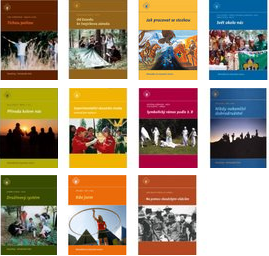
\includegraphics[width=4cm]{prirucky.png}
  \end{center}
\end{frame}

\begin{frame}{Na čem právě pracujeme (v~různé fázi)}
  \begin{center}
    
\includegraphics[width=2cm]{lilie.png}
  \end{center}
  \begin{itemize}
    \item Revize kompetencí a~stezek --- jak se osvědčily, co zlepšit
    \item Doplňky ke stezce, příručky
    \item Doplňky programu pro vlčata a~světlušky (mladší školní věk)
    \item Předškolní věk („benjamínci“), rodinný skauting, inkluzivní skauting pro znevýhodněné (nějak hendikepované, sociálně slabé,~\ldots), lepší vzdělávání dospělých,~\ldots
    \item Lepší zapojení oldskautů, lepší personalistika (neztrácet lidský potenciál)
    \item Využití dostupných statistických a~sociologických dat
    \item A~další\ldots
  \end{itemize}
\end{frame}

\subsection{Zdroje informací}

\begin{frame}[allowframebreaks]{Další informace}
  \begin{itemize}
    \item Informace o~skautském výchovném programu: \url{https://krizovatka.skaut.cz/organizace/vzdelavani/vzdelavaci-system} a~\url{https://krizovatka.skaut.cz/oddil/program}
    \begin{itemize}
      \item Materiály ke stažení
      \item Informace o~seminářích, kurzech,~\ldots
      \item Databáze programů
      \item Řada dalších informací\ldots
    \end{itemize}
    \item Web pro veřejnost: \url{https://www.skaut.cz/}
    \item Časopisy elektronicky: \url{https://casopisy.skaut.cz/}
    \item Knihy \textbf{Skautské století} (Roman Šantora, Václav Nosek, Slavomil Janov a~Václav Dostál, TDC a~Mladá fronta, 2012), \textbf{Skautský oddíl 1913--2013} (Roman Šantora a kol., TDC a Mladá fronta, 2014) a \href{https://www.obchod.skaut.cz/publikace/}{další} a \href{https://www.junshop.cz/Tiskoviny-a-DVD/}{další}
    \item Skautský institut: \url{https://www.skautskyinstitut.cz/} (vzdělávání, historie skautingu, akce pro veřejnost)
    \item Budete-li mít v~budoucnu dotazy, klidně se mi ozvěte a~zeptejte se, \url{https://trapa.cz/cs/kontakt}, \href{https://krizovatka.skaut.cz/organizace/ustredi/odbory/ekoodbor}{http://skaut.cz/eko}
  \end{itemize}
\end{frame}

\begin{frame}{Děkuji za pozornost\ldots}
  \begin{center}
    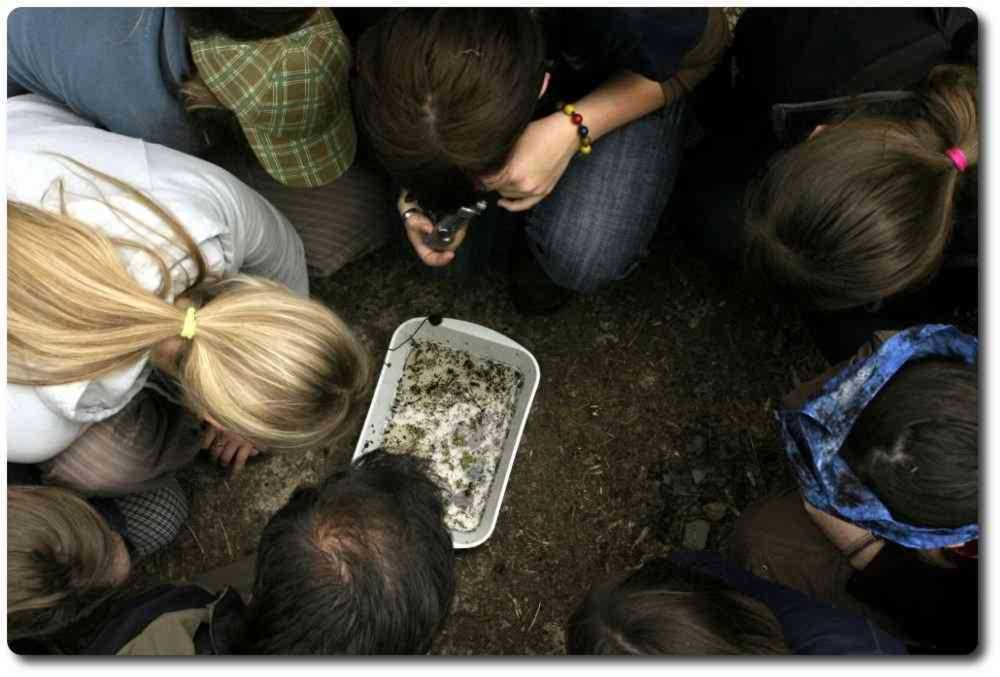
\includegraphics[height=6cm]{zaver.jpg}
  \end{center}
  \begin{flushright}
    \begin{large}
      \ldots otázky?
    \end{large}
  \end{flushright}
\end{frame}

\end{document}
